% =============================================================================
% =============================================================================
% CAPÍTULOS 3, 4, 5, 6, 7 --- ETAPA 2 (a produzir após validação da Etapa 1)
% =============================================================================
% =============================================================================

% =============================================================================
% TESE DE DOUTORADO — BioRemPP — ETAPA 2
% Bioremediation Potential Profiling
% Programa de Pós-Graduação em Bioinformática — UFRN
%
% =============================================================================
% INSTRUÇÕES DE INTEGRAÇÃO NO ARQUIVO PRINCIPAL (tese_biorempp_etapa1.tex):
%
% 1. Abrir o arquivo tese_biorempp_etapa1.tex.
% 2. Localizar a linha que começa com "\chapter{Componente 1: Banco de dados"
%    (aproximadamente linha 660 do arquivo original).
% 3. DELETAR do início dessa linha até imediatamente ANTES da linha
%    "\end{document}" (a última linha do arquivo).
% 4. COLAR o conteúdo deste arquivo (tudo abaixo desta caixa de instruções)
%    exatamente no ponto onde a linha "\chapter{Componente 1: ..." estava.
% 5. A linha "\end{document}" deve permanecer no arquivo principal, sem
%    duplicação.
%
% RESULTADO: o arquivo principal fica com preâmbulo + pré-textuais + Cap 1 +
% Cap 2 (Etapa 1) + Cap 3–7 + referências + apêndices (Etapa 2) + \end{document}.
% =============================================================================


% =============================================================================
% =============================================================================
% CAPÍTULO 3 --- COMPONENTE 1: BANCO DE DADOS INTEGRADO E PIPELINE DE GERAÇÃO
% =============================================================================
% =============================================================================
\chapter{Componente 1: Banco de dados integrado e pipeline de geração}
\label{cap:comp1}

% -----------------------------------------------------------------------------
\section{Motivação do componente}
\label{sec:c1-motivacao}
% -----------------------------------------------------------------------------

O primeiro componente do ecossistema \biorempp{} é o substrato de evidência sobre o qual os demais operam. Enquanto \gls{kegg}, \gls{hadeg}, \gls{toxcsm} e as listas regulatórias oferecem, cada um, coberturas específicas de conhecimento relevantes para biorremediação, nenhuma dessas fontes por si só suporta a análise \textit{compound-centric} orientada a prioridade regulatória que motivou este trabalho. A construção do banco integrado responde a essa lacuna consolidando, em um único artefato curado e versionado, as evidências funcionais, toxicológicas e regulatórias associadas aos compostos ambientalmente prioritários.

A decisão editorial central deste componente é restritiva por desígnio: em vez de acumular a totalidade dos compostos disponíveis em cada fonte, o banco projeta as evidências das quatro fontes sobre o universo de compostos formalmente listados por sete frameworks regulatórios internacionais e regionais. Essa restrição faz do banco não uma agregação exaustiva, mas uma curadoria com propósito, cuja utilidade emerge exatamente do recorte adotado.

O pipeline que gera o banco e as camadas de validação que o auditam são apresentados neste mesmo capítulo porque, do ponto de vista da contribuição científica, formam uma unidade indissociável do artefato de dados: a reprodutibilidade e a auditabilidade do release são propriedades técnicas do banco, não externalidades operacionais.

% -----------------------------------------------------------------------------
\section{Fontes de dados consolidadas}
\label{sec:c1-fontes}
% -----------------------------------------------------------------------------

Nesta tese, a expressão ``fontes consolidadas'' opera em dois níveis complementares. No primeiro, o banco parte de um universo regulatório de compostos prioritários definido por sete frameworks e jurisdições regulatórias, operacionalizados em nove códigos no campo \texttt{referenceAG} devido ao desdobramento da \gls{iarc} em três categorias. No segundo, esse universo curado recebe as camadas funcionais e toxicológicas integradas no release v1.1.0. Conforme descrito em \texttt{online\_methods.tex}, a gênese desse recorte foi \textit{regulatory-driven}: os compostos foram inicialmente coletados a partir de listas regulatórias, identificados por nome químico e \gls{cas}, submetidos à expansão de sinônimos e mantidos apenas quando houve mapeamento inequívoco para identificadores químicos externos, em especial PubChem CID ou ChEBI.

\begin{table}[htbp]
\centering
\caption{Origem regulatória do universo de compostos prioritários do \biorempp{}. A tabela adapta a síntese histórica de \texttt{online\_methods.tex} ao vocabulário controlado atual do campo \texttt{referenceAG}.}
\label{tab:c1-regulatory-sources}
\footnotesize
\begin{tabularx}{\textwidth}{@{}lXlX@{}}
\toprule
\textbf{Código no release} & \textbf{Agência / framework} & \textbf{Escopo geográfico} & \textbf{Papel no recorte regulatório} \\
\midrule
ATSDR & Agency for Toxic Substances and Disease Registry & EUA & Prioriza substâncias associadas a risco em saúde pública e sítios contaminados. \\
EPA & U.S. Environmental Protection Agency & EUA & Introduz contaminantes prioritários e referências de qualidade ambiental e hídrica. \\
CONAMA & Conselho Nacional do Meio Ambiente & Brasil & Representa normas ambientais nacionais para contaminantes relevantes no contexto brasileiro. \\
WFD & Water Framework Directive & União Europeia & Delimita substâncias prioritárias ligadas à qualidade de águas superficiais e subterrâneas. \\
EPC & Environmental Priority Chemicals & Europa / União Europeia & Complementa o recorte europeu com substâncias priorizadas em ambientes aquáticos. \\
PSL & Priority Substances List (sob CEPA) & Canadá & Introduz substâncias de preocupação regulatória no contexto canadense. \\
IARC1 & IARC Group 1 --- Carcinogenic to humans & Internacional & Marca compostos com evidência estabelecida de carcinogenicidade humana. \\
IARC2A & IARC Group 2A --- Probably carcinogenic to humans & Internacional & Marca compostos com evidência provável de carcinogenicidade humana. \\
IARC2B & IARC Group 2B --- Possibly carcinogenic to humans & Internacional & Marca compostos com evidência possível de carcinogenicidade humana. \\
\bottomrule
\end{tabularx}
\end{table}

Esses frameworks definem o universo inicial de compostos prioritários sobre o qual o banco é construído. Na formulação histórica resumida em \texttt{online\_methods.tex}, esse universo foi curado com apoio de \gls{cas}, nomes químicos e expansão de sinônimos para maximizar a recuperação de identificadores resolvíveis. Na implementação atual, o resultado consolidado dessa etapa entra no pipeline como pares normalizados \texttt{cpd} + \texttt{referenceAG}, preservados principalmente em \texttt{curated\_regulated\_compounds.xlsx}, que ancora o espaço inicial de compostos e a proveniência regulatória do release.

Sobre esse universo regulatório curado, o release v1.1.0 integra quatro fontes primárias, cada uma contribuindo com um tipo específico de evidência (Tabela~\ref{tab:c1-fontes}).

\begin{table}[htbp]
\centering
\caption{Fontes primárias integradas ao banco \biorempp{} no release v1.1.0 e respectivas chaves de ligação ao núcleo relacional.}
\label{tab:c1-fontes}
\small
\begin{tabular}{@{}lrrl@{}}
\toprule
\textbf{Fonte} & \textbf{Linhas} & \textbf{Colunas} & \textbf{Chave} \\
\midrule
BioRemPP core        & 123.543 & 11 & \gls{ko}, \gls{cpd} \\
HADEG                &    867 &  4 & \gls{ko} \\
KEGG Degradation     &    855 &  3 & \gls{ko} \\
ToxCSM               &    370 & 66 & \gls{cpd} \\
\bottomrule
\end{tabular}
\end{table}

A \textbf{tabela core BioRemPP} é o esqueleto relacional que carrega as associações entre compostos, orthologs, enzimas, reações e agências regulatórias. Cada registro conecta um composto (\texttt{cpd}, \texttt{compoundname}, \texttt{compoundclass}) a uma unidade funcional (\texttt{ko}, \texttt{genesymbol}, \texttt{genename}, \texttt{enzyme\_activity}) através de uma transformação enzimática específica (\texttt{ec}, \texttt{reaction}, \texttt{reaction\_description}), com âncora regulatória no campo \texttt{referenceAG}.

Essas quatro fontes integradas não se confundem com os arquivos curados locais consumidos pelo pipeline. Os arquivos \texttt{curated\_regulated\_compounds.xlsx} e \texttt{curated\_programatic\_missing\_compounds.xlsx} definem o espaço inicial de chaves \texttt{cpd}, \texttt{ko} e \texttt{referenceAG}; \texttt{curated\_compound\_classes.xlsx} determina \texttt{compoundclass}; \texttt{kegglistko.txt} fornece \texttt{genesymbol} e \texttt{genename}; e \texttt{curated\_enzyem\_names\_extracted.txt} ancora a extração de \texttt{enzyme\_activity}. O arquivo \texttt{kegglistcompounds.xlsx} permanece no contrato de entrada, mas o campo público \texttt{compoundname} é preenchido pela lista de compostos do KEGG na implementação ativa do release v1.1.0.

A \textbf{HADEG}~\citep{rojas2023hadeg} contribui com evidência especializada em degradação aeróbica de hidrocarbonetos: 323 símbolos gênicos únicos, 337 \glspl{ko} e 71 vias metabólicas distribuídas em cinco classes de hidrocarbonetos (Alcanos, Aromáticos, Alcenos, Cicloalcanos e BTEX). A profundidade de resolução por via alcançada pela HADEG em seu domínio-alvo não é replicada pelas anotações genéricas de xenobióticos do KEGG.

O \textbf{KEGG Degradation}~\citep{kanehisa2022kegg} é uma extração focada da branch de metabolismo de xenobióticos do KEGG, contendo 517 \glspl{ko} distribuídos em 20 vias canônicas (Naftaleno, Benzoato, Aminobenzoato, Cloroalcano, Atrazina, Bisfenol, Aromáticos policíclicos, entre outras). Esta fonte fornece o esqueleto canônico de metabolismo xenobiótico do recurso integrado.

O \textbf{ToxCSM}~\citep{desa2022toxCSM} fornece perfis toxicológicos preditos por modelos \gls{qsar} para 370 dos 384 compostos do banco (96,4\% de cobertura). Cada composto carrega 31 predições de endpoint, cada uma desdobrada em uma etiqueta categórica (\textit{Safety}, \textit{Moderate Risk}, \textit{High Risk}) e um escore contínuo no intervalo $[0, 1]$. Os endpoints estão organizados em cinco categorias: ambiental (6 endpoints, incluindo aviária, crustáceos, peixes, polinizadores, protozoários e biodegradação predita), genômica (3, incluindo mutagênese AMES, carcinogênese e formação de micronúcleos), toxicidade orgânica (8, incluindo hepatotoxicidade, cardiotoxicidade via hERG e efeitos oculares e dérmicos), ligação a receptores nucleares (9, cobrindo AhR, AR, AR-LBD, ER, ER-LBD, aromatase, GR, PPAR-$\gamma$ e TR) e ativação de resposta ao estresse (5, incluindo ARE, ATAD5, HSE, MMP e p53). O endpoint \textit{Biodegradation} do ToxCSM estima persistência ambiental por \gls{qsar} e, portanto, é conceitualmente distinto da evidência de biodegradação biológica curada nas camadas funcionais do banco.

% -----------------------------------------------------------------------------
\section{Modelo de integração dual-axis}
\label{sec:c1-dualaxis}
% -----------------------------------------------------------------------------

As quatro fontes são conectadas por meio de duas chaves de integração complementares que operam simultaneamente sobre o banco core (Figura~\ref{fig:c1-dualaxis}). O eixo \textbf{funcional} usa o identificador \gls{ko} para ligar a tabela core BioRemPP, o HADEG e o KEGG Degradation, permitindo que um único ortholog acumule evidência proveniente de metabolismo xenobiótico canônico, vias específicas de hidrocarbonetos e associações composto-gene-enzima da curadoria interna. O eixo \textbf{químico} usa o identificador \gls{cpd} (KEGG Compound) para ligar a tabela core ao ToxCSM, anexando as predições toxicológicas aos registros de compostos.

O pipeline aplica três modelos de evidência em ordem decrescente de completude. No modelo \textit{ko\_complete}, o par composto--KO é expandido por relações KEGG suficientemente densas para resolver simultaneamente \texttt{ec} e \texttt{reaction}. No modelo \textit{ko\_fallback}, apenas parte dessa estrutura relacional está disponível, preservando a associação funcional mesmo quando uma das duas colunas permanece nula. No modelo \textit{compound\_bridge}, pares \texttt{cpd}--\texttt{ko} oriundos de curadoria programática são mantidos apesar de o KEGG não fechar diretamente o circuito completo de links. As nulabilidades de \texttt{ec} e \texttt{reaction} são, portanto, representação explícita da completude da evidência, e não defeito de preenchimento.

\begin{figure}[htbp]
\centering
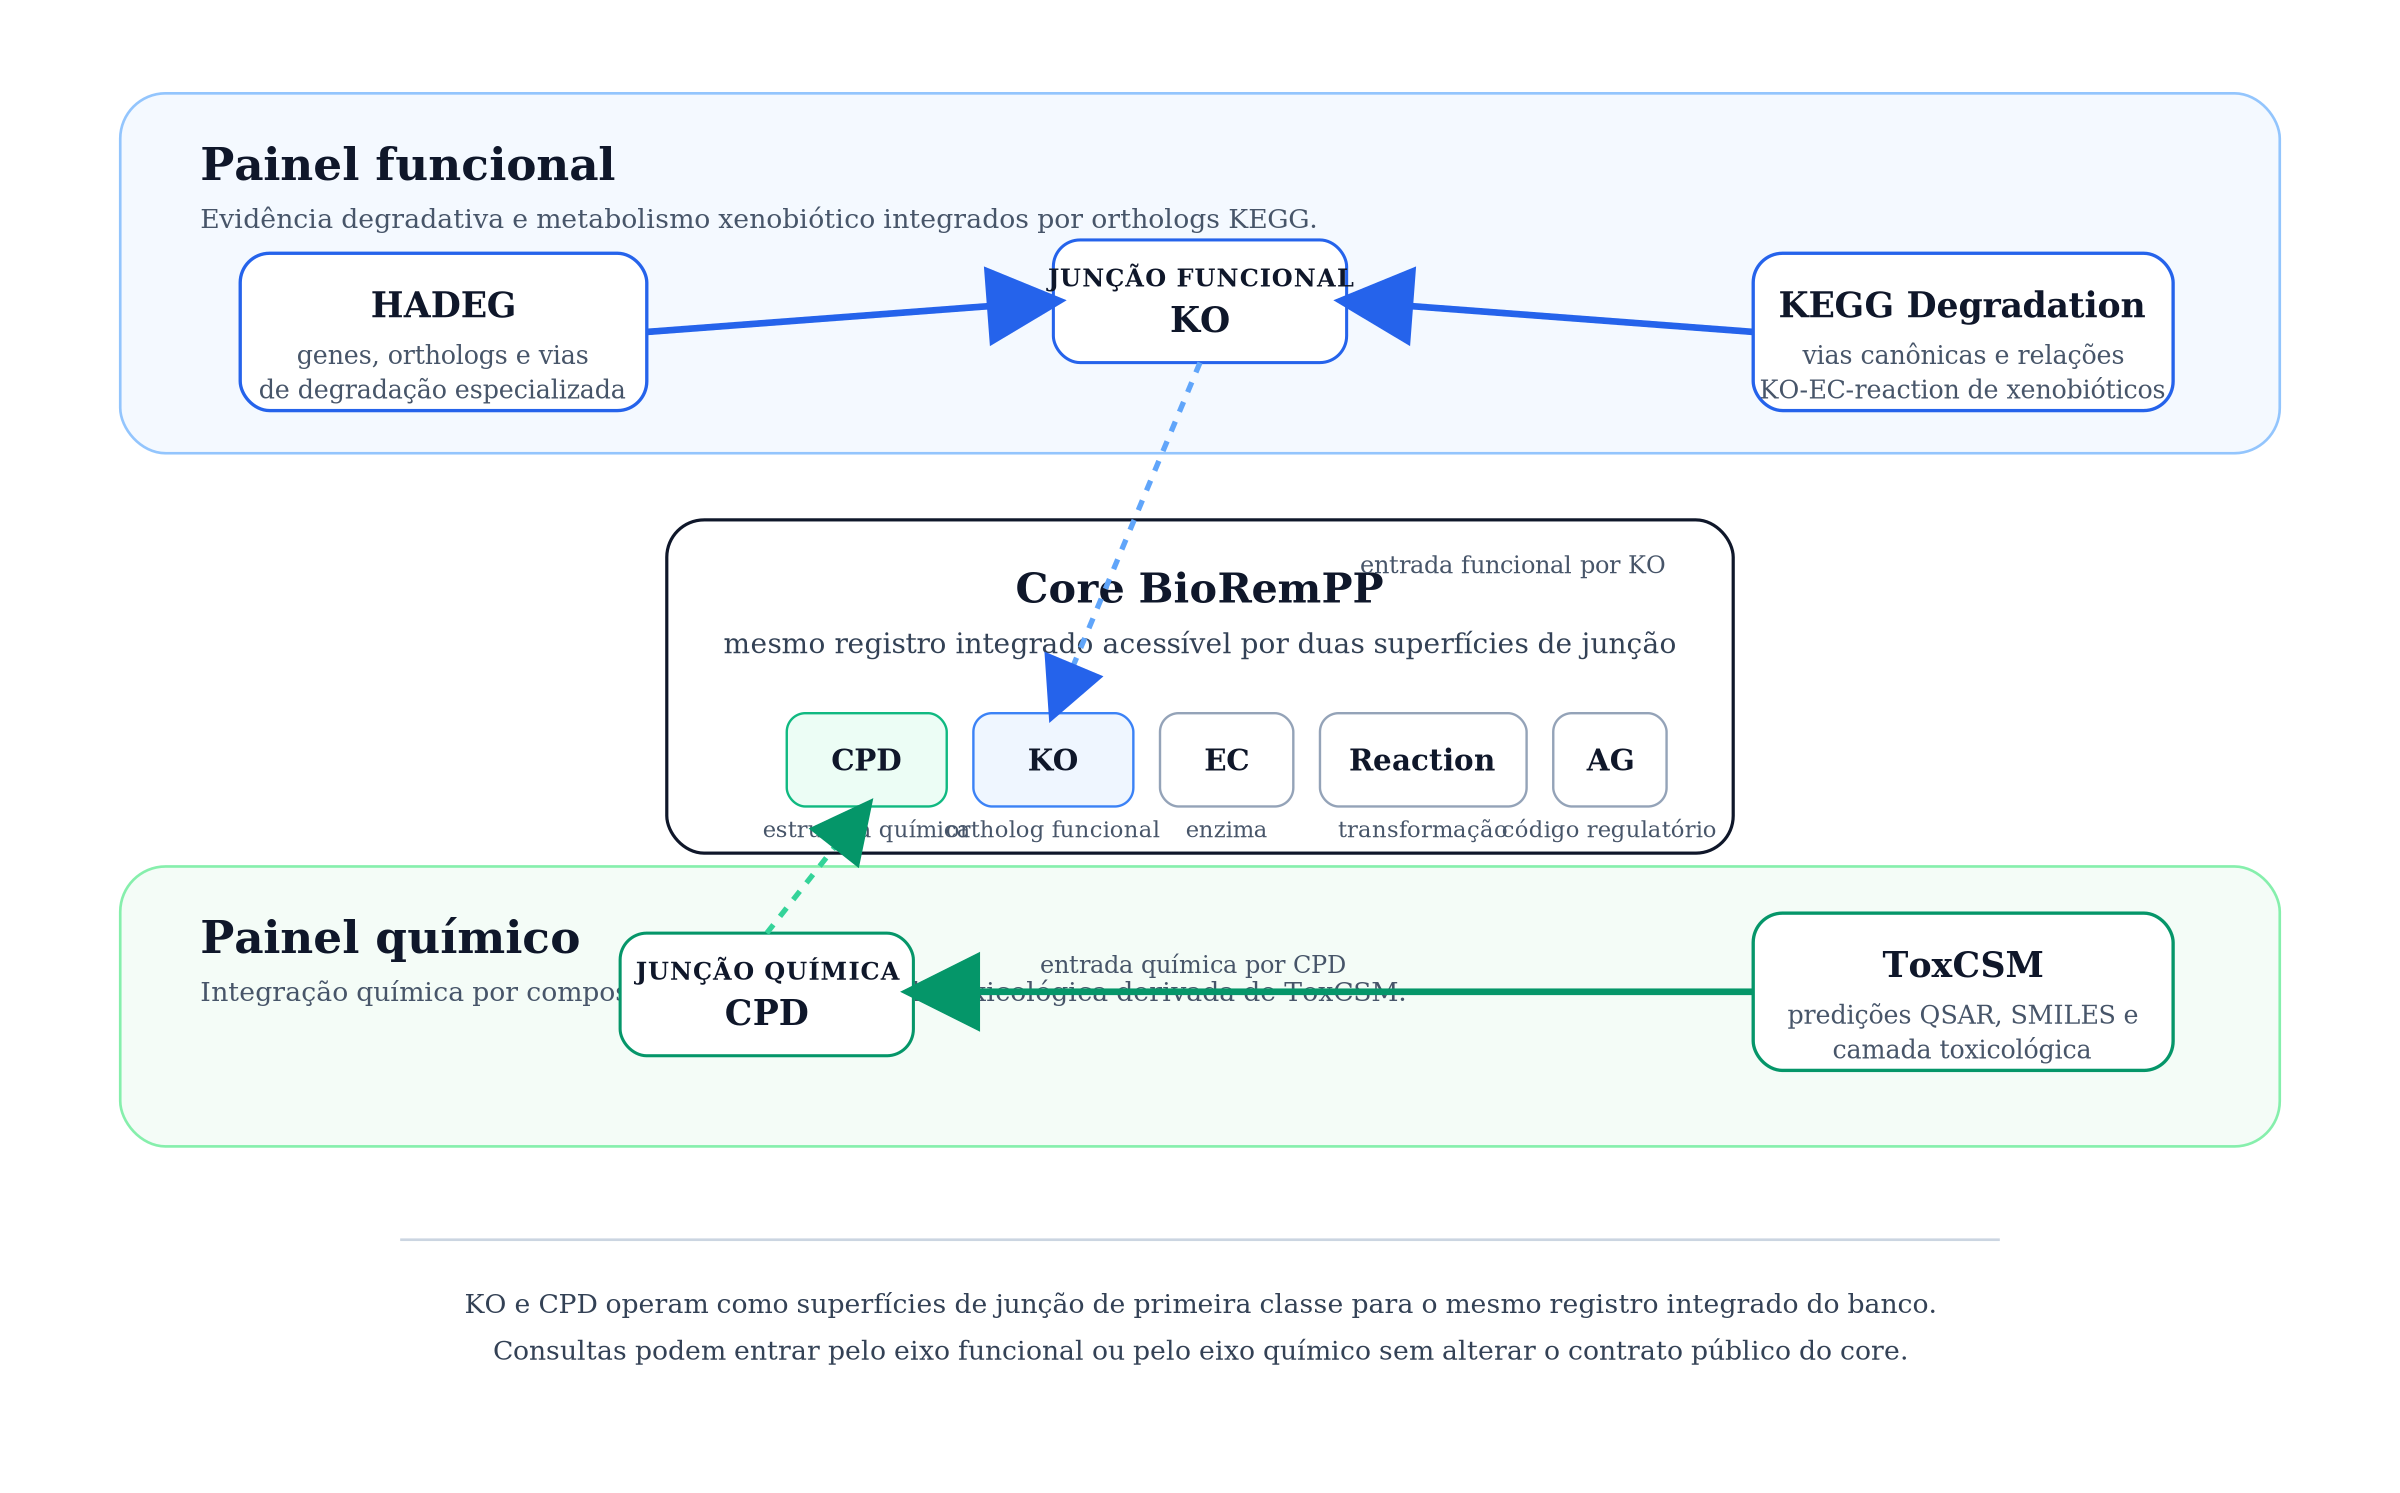
\includegraphics[width=\textwidth]{figures/chapter_03/fig_03_01_dual_axis.png}
\caption{Modelo de integração dual-axis do banco \biorempp{}. O eixo funcional (\gls{ko}) e o eixo químico (\gls{cpd}) operam como superfícies de junção de primeira classe, permitindo que consultas entrem no grafo integrado por qualquer uma das duas dimensões.}
\label{fig:c1-dualaxis}
\end{figure}

A adoção de duas chaves de integração paralelas, em vez de uma única, reflete uma assimetria estrutural na biologia subjacente: a atividade enzimática é naturalmente indexada por ortholog, enquanto a predição de toxicidade é naturalmente indexada por estrutura molecular. Forçar todas as fontes através de um único identificador ou obscureceria a riqueza funcional das fontes indexadas por \gls{ko}, ou exigiria um mapeamento ontológico entre \gls{ko} e \gls{cpd} que não existe na taxonomia KEGG. O modelo dual-axis trata ambas as dimensões como superfícies de junção de primeira classe e permite que consultas entrem no grafo integrado a partir de qualquer um dos dois lados sem ambiguidade.

% -----------------------------------------------------------------------------
\section{Schema e identificadores interoperáveis}
\label{sec:c1-schema}
% -----------------------------------------------------------------------------

A tabela core BioRemPP é organizada em 11 campos semânticos ordenados (Tabela~\ref{tab:c1-schema}), armazenados em CSV com codificação UTF-8, delimitador ponto-e-vírgula e qualificador de texto por aspas duplas. No release v1.1.0, esse contrato público contém 123.543 linhas e 11 colunas. Todos os identificadores utilizados são herdados de autoridades externas públicas, com validação de formato aplicada em tempo de construção.

\begin{table}[htbp]
\centering
\caption{Schema da tabela core BioRemPP (v1.1.0). Campos com nulabilidade explícita usam sentinelas \texttt{NA} em vez de \textit{silent backfill}.}
\label{tab:c1-schema}
\small
\begin{tabularx}{\textwidth}{@{}llX@{}}
\toprule
\textbf{Campo} & \textbf{Tipo} & \textbf{Descrição} \\
\midrule
\texttt{cpd}                  & Caractere & KEGG Compound identifier (\texttt{\^{}C\textbackslash d\{5\}\$}) \\
\texttt{compoundclass}        & Caractere & Classe química (12 valores controlados) \\
\texttt{ko}                   & Caractere & KEGG Orthology identifier (\texttt{\^{}K\textbackslash d\{5\}\$}) \\
\texttt{ec}                   & Caractere & Enzyme Commission number (nulável) \\
\texttt{reaction}             & Caractere & KEGG Reaction identifier (\texttt{\^{}R\textbackslash d\{5\}\$}, nulável) \\
\texttt{reaction\_description}& Caractere & Descrição textual da reação (nulável) \\
\texttt{referenceAG}          & Caractere & Código da agência regulatória (9 valores) \\
\texttt{compoundname}         & Caractere & Nome do composto \\
\texttt{genesymbol}           & Caractere & Símbolo gênico \\
\texttt{genename}             & Caractere & Nome do gene \\
\texttt{enzyme\_activity}     & Caractere & Família de atividade enzimática (206 valores) \\
\bottomrule
\end{tabularx}
\end{table}

A adoção de identificadores externos como chaves primárias é uma decisão de design consciente que assegura interoperabilidade sem custo adicional. Nenhum identificador é específico do BioRemPP: \texttt{cpd} resolve para KEGG Compound, \texttt{ko} para KEGG Orthology, \texttt{reaction} para KEGG Reaction, \texttt{ec} para \gls{ec}, e a coluna análoga \texttt{ChEBI} do subconjunto ToxCSM resolve para EMBL-EBI ChEBI. As estruturas moleculares (\gls{smiles}) são armazenadas verbatim como representações machine-readable diretamente consumíveis por toolkits de quimioinformática. Essa escolha assegura conformidade com os princípios \gls{fair} (Seção~\ref{sec:fund-fair}) e portabilidade para pipelines multi-ômicos externos. No mesmo espírito, as colunas \texttt{ec}, \texttt{reaction} e \texttt{reaction\_description} permanecem semanticamente nuláveis: o pipeline serializa \texttt{NA} quando a resolução do KEGG não sustenta preenchimento confiável, em vez de recorrer a \textit{backfill} silencioso.

\subsection{Denormalização e evolução do row count entre releases}

A tabela core adota schema plano e denormalizado. Essa decisão prioriza usabilidade em ferramentas tabulares (R \texttt{readr}, Python \texttt{pandas}, planilhas) sobre eficiência de armazenamento, e tem como consequência que o número de linhas reflete a superfície relacional expandida em vez do inventário de entidades subjacente. Entre as releases v1.0.0 (10.871 linhas; release de dezembro de 2023) e v1.1.0 (123.543 linhas; KEGG Release 118.0+, recuperado em 18 de maio de 2026) houve expansão de aproximadamente onze vezes, decorrente da introdução das colunas \texttt{ec}, \texttt{reaction} e \texttt{reaction\_description} e da correspondente enumeração de combinações EC--reação suportadas pelo KEGG. Um único par composto--KO que antes ocupava uma linha no contrato de oito colunas passa a gerar uma linha por combinação distinta de \texttt{ec} e \texttt{reaction} no contrato atual de 11 colunas. As cardinalidades entity-level (384 compostos, 1.543 \glspl{ko} únicos, 994 números EC e 1.939 identificadores de reação KEGG) permanecem sendo as métricas cientificamente relevantes.

% -----------------------------------------------------------------------------
\section{Pipeline Snakemake}
\label{sec:c1-snakemake}
% -----------------------------------------------------------------------------

O banco integrado é produzido por um workflow Snakemake~\citep{molder2025snakemake} organizado em torno de um \gls{dag} explícito, cujo contrato de release e dependências entre estágios são declarados e versionados junto com os dados que gera.

\subsection{Arquitetura em quatro camadas}

O workflow separa deliberadamente quatro responsabilidades em camadas distintas:

\begin{description}
    \item[Camada de orquestração:] \texttt{Snakefile} e cinco módulos de \textit{rules} (\texttt{00\_preflight}, \texttt{10\_generation}, \texttt{20\_analysis}, \texttt{30\_validation}, \texttt{90\_reporting}) declaram quais artefatos pertencem a uma release completa e quais dependências devem estar satisfeitas antes de cada regra executar. A camada de orquestração não contém lógica de transformação.
    \item[Camada de contrato:] \texttt{config/config.yaml} armazena valores de runtime (versão, caminhos, formato CSV, endpoints KEGG, thresholds de validação); \texttt{workflow/lib/io\_contracts.R} armazena o contrato estrutural (nomes obrigatórios de arquivos curados, vetor ordenado de 11 colunas do schema exportado, padrões regex de identificadores, endpoints KEGG usados pela geração).
    \item[Camada de scripts:] transformações efetivas implementadas em \texttt{workflow/scripts/}, agrupadas por estágio, com scripts que leem inputs declarados e escrevem outputs declarados sem orquestrarem uns aos outros diretamente.
    \item[Camada de utilidades:] \texttt{workflow/lib/utils.R} concentra funções compartilhadas (I/O CSV/JSON, normalização de sentinelas NA, logging, parsing de argumentos de linha de comando).
\end{description}

Essa separação garante que decisões operacionais que mudam entre releases (caminhos, thresholds) sejam ajustadas via YAML sem alteração de código, enquanto mudanças no que constitui \textit{um release do banco BioRemPP} (schema, regras de identificadores) sejam mudanças de código com histórico auditável em version control.

\subsection{Estágios de execução da release}

A Tabela~\ref{tab:c1-stages} resume os dez estágios do \gls{dag}. A ordem é lógica, não estritamente sequencial: o Snakemake agenda regras independentes em paralelo sempre que suas dependências declaradas já estão satisfeitas.

\begin{table*}[htbp]
\centering
\caption{Estágios do \gls{dag} de release do pipeline \biorempp{}.}
\label{tab:c1-stages}
\small
\begin{tabular}{@{}rlll@{}}
\toprule
\textbf{\#} & \textbf{Estágio} & \textbf{Regra(s) principal(is)} & \textbf{Artefato principal} \\
\midrule
1  & Preflight               & \texttt{preflight\_check\_inputs}             & \texttt{work/preflight\_ok.json} \\
2  & Bundle local curado     & \texttt{load\_local\_data}                    & \texttt{work/local\_data.rds} \\
3  & Aquisição KEGG          & \texttt{fetch\_kegg\_info}, \texttt{fetch\_kegg\_data} & \texttt{results/metadata/kegg\_release.json}, \texttt{work/kegg\_data.rds} \\
4  & Assembly de relações    & \texttt{merge\_relationships}       & \texttt{work/merged\_compounds.rds} \\
5  & Classificação           & \texttt{add\_classifications}       & \texttt{work/classified\_compounds.rds} \\
6  & Enriquecimento gênico   & \texttt{enrich\_gene\_info}         & \texttt{work/enriched\_compounds.rds} \\
7  & Exportação da release   & \texttt{extract\_enzymes\_export}   & \texttt{biorempp\_database\_v1.1.0.\{csv,xlsx\}} \\
8  & Análise                 & 9 regras                            & \texttt{results/analysis/*.json} \\
9  & Validação integrada     & 3 regras                            & \texttt{results/metadata/*\_report.json} \\
10 & Relatório final         & \texttt{build\_run\_report}         & \texttt{results/reports/workflow\_summary.json} \\
\bottomrule
\end{tabular}
\end{table*}

\begin{figure}[htbp]
\centering
\fbox{\parbox{0.85\textwidth}{\centering Representação esquemática do \gls{dag} do release BioRemPP, com nós para regras e arestas para dependências de artefatos. O desenho distingue os módulos de preflight, geração, análise, validação integrada e relatório final.\vspace{2em}}}
\caption{Grafo de dependências do pipeline Snakemake do banco \biorempp{}, agrupado pelos cinco módulos de \textit{rules}. Setas indicam a direção de propagação de artefatos.}
\label{fig:c1-dag}
\end{figure}

Os estágios 4 a 7 concentram a construção iterativa da tabela integrada. Em \texttt{merge\_relationships}, o pipeline combina o bundle local curado (\texttt{work/local\_data.rds}) com o bundle KEGG (\texttt{work/kegg\_data.rds}) para formar o universo \texttt{cpd}--\texttt{ko}--\texttt{referenceAG} e expandi-lo segundo as relações disponíveis entre compostos, orthologs, ECs e reações. O resultado desse estágio é serializado em \texttt{work/merged\_compounds.rds}, tornando explícito o estado relacional antes da classificação química.

Em \texttt{add\_classifications}, as classes químicas curadas são anexadas ao objeto intermediário, com normalização de vocabulário e expansão de compostos que carregam múltiplas classes. O estado enriquecido é persistido em \texttt{work/classified\_compounds.rds}. Em \texttt{enrich\_gene\_info}, o pipeline junta \texttt{genesymbol} e \texttt{genename} oriundos de \texttt{kegglistko.txt}, produzindo \texttt{work/enriched\_compounds.rds} como último bundle intermediário antes da exportação pública.

No estágio \texttt{extract\_enzymes\_export}, o objeto enriquecido recebe \texttt{enzyme\_activity} por meio de regex curada sobre \texttt{genename}, incorpora \texttt{reaction\_description} a partir de \texttt{list/reaction} do KEGG e é então exportado nos contratos públicos \texttt{CSV} e \texttt{XLSX}. A serialização de cada estado intermediário em bundles \texttt{.rds} permite reruns parciais, inspeção de fronteiras entre estágios e auditoria de transformações sem depender de reconstrução integral do \gls{dag}.

% -----------------------------------------------------------------------------
\section{Validação KEGG-anchored embutida}
\label{sec:c1-validacao-kegg}
% -----------------------------------------------------------------------------

A primeira camada de validação está embutida no \gls{dag} Snakemake (estágio 9) e audita o banco exportado contra o grafo de links do próprio KEGG. Antes de avaliar o banco, o pipeline persiste um cache local dos payloads KEGG relevantes (regra \texttt{fetch\_kegg\_link\_cache} $\rightarrow$ arquivos TSV em \texttt{cache/kegg\_link\_cache/}), assegurando que a validação opere reproduzivelmente contra um snapshot fixo do KEGG em vez de re-consultar a API a cada execução.

Duas regras de relatório então avaliam o banco exportado contra esse ground truth cacheado:

\begin{description}
    \item[\texttt{validate\_keys\_consistency} $\rightarrow$ \texttt{keys\_consistency\_report.json}] endereça as linhas do banco exportado que carregam sentinela \texttt{NA} em \texttt{ec} ou \texttt{reaction}. Classifica cada linha como \textit{justificada} (nenhum link KEGG existe para o par \texttt{ko}-\texttt{cpd} correspondente, portanto a ausência é correta) ou \textit{incorreta} (um link KEGG existe, portanto o estágio de expansão cartesiana deveria ter materializado uma linha populada). A proporção de linhas \textit{justificadas} versus \textit{incorretas} é o indicador de qualidade principal desse relatório: uma taxa próxima a 100\% de justificadas significa que \texttt{ec} ou \texttt{reaction} vazios refletem lacunas reais do KEGG em vez de erros de build.

    \item[\texttt{validate\_links\_groundtruth\_policy} $\rightarrow$ \texttt{links\_groundtruth\_policy\_report.json}] endereça as linhas que carregam \texttt{ec} e \texttt{reaction} populados. Mede a concordância pair-level entre as combinações \texttt{(ko, ec, reaction)} no banco exportado e o grafo de links KEGG capturado no cache, quantificando cobertura policy-aware. O threshold \texttt{validation.max\_invalid\_line\_ratio} em \texttt{config/config.yaml} define a taxa máxima aceitável de discordância para o release passar.
\end{description}

Essa camada é propositalmente construída para o conteúdo KEGG-ancorado do banco e trata o snapshot de links KEGG capturado no release como referência operacional. Sua semântica é predominantemente \textit{report-oriented}: falhas de aquisição do cache, parsing inválido, ausência de arquivos obrigatórios ou violação do threshold configurado podem interromper a execução, mas os achados row-level são persistidos como artefatos diagnósticos em JSON, permitindo revisão explícita da release em vez de absorção silenciosa.

Na release v1.1.0, os relatórios integrados registraram 123.543 linhas no banco, das quais 3.111 apresentaram algum \texttt{NA} em \texttt{ec} ou \texttt{reaction}. Todas as 3.111 ocorrências foram classificadas como justificadas, e nenhuma foi classificada como incorreta. Entre as 120.432 linhas densas avaliadas na política de ground truth, a taxa \texttt{policy\_union} foi de 100,0\%, indicando que toda linha com \texttt{ec} e \texttt{reaction} preenchidos encontra suporte em pelo menos um dos modelos de evidência admitidos pela política ativa. A taxa \texttt{strict5} foi de 2,42\%, refletindo um critério deliberadamente conservador que exige suporte simultâneo das cinco relações KEGG cacheadas e, portanto, não deve ser interpretado como veredito global de qualidade.

% -----------------------------------------------------------------------------
\section{Validação Great Expectations release-level}
\label{sec:c1-validacao-gx}
% -----------------------------------------------------------------------------

A segunda camada de validação, implementada em projeto separado sob \texttt{biorempp\_validation/}, opera com \gls{gx}~\citep{greatexpectations} e consome a árvore de resultados finalizada após o Snakemake concluir. Diferente da camada KEGG-anchored, a validação Great Expectations pergunta questões estruturais e de estabilidade: o banco exportado tem o schema que o contrato declara? Seus identificadores respeitam os padrões regex? Os artefatos de análise concordam com o banco que descrevem? A release atual permanece consistente com o comportamento analítico da baseline commitada? O entrypoint \texttt{biorempp-validate} executa cinco etapas: carrega as configurações, realiza preflight dos artefatos correntes e da baseline quando necessário, lê o CSV e os JSONs relevantes, materializa \texttt{DataFrames} derivados e, por fim, executa as suites configuradas. Em todo o processo, o validador é read-only em relação às saídas do Snakemake.

\subsection{Justificativa da arquitetura dual}

Nenhuma das camadas isoladamente é suficiente. Um release que passa apenas na validação KEGG-anchored pode estar silenciosamente quebrado em ordem de colunas, formatos de identificador ou valores de vocabulário controlado; um release que passa apenas na validação Great Expectations pode conter anotações \texttt{ec} ou \texttt{reaction} que discordam do KEGG. A combinação das duas camadas responde afirmativamente, para cada release, a duas perguntas distintas: o conteúdo é fiel às fontes upstream, e o artefato está corretamente estruturado segundo seu próprio contrato.

\subsection{Modos ortogonais de validação}

O validador expõe dois modos controlando quais suites de comparação analítica executam. Os modos são ortogonais: podem ser habilitados juntos ou independentemente, e as suites estruturais e de metadata KEGG executam independentemente dos modos ativos.

\begin{itemize}
    \item \textbf{Internal-consistency:} compara o CSV da release atual contra seus próprios artefatos de análise. Verifica se as contagens, distribuições e sumários da família JSON (\texttt{basic\_statistics.json}, \texttt{compound\_statistics.json}, etc.) concordam com o que pode ser recomputado a partir do CSV. Endereça o modo de falha em que o estágio de análise reporta métricas que não correspondem ao banco descrito.

    \item \textbf{Regression-detection:} compara o CSV da release atual contra uma baseline commitada sob \texttt{baselines/release\_v1\_1\_0\_kegg\_118\_0plus} no repositório. Endereça o modo de falha em que uma release futura silenciosamente altera uma métrica derivada que deveria permanecer estável.
\end{itemize}

\subsection{Suites de expectativas}

Oito arquivos JSON de suite acompanham o validador. Em tempo de execução, um deles serve como template clonado em duas suites concretas (uma por modo de comparação analítica), totalizando nove identidades de suite ativas (Tabela~\ref{tab:c1-suites}).

\begin{table*}[htbp]
\centering
\caption{Suites de expectativas do validador \gls{gx} release-level. Mode indica se a suite executa sempre (agnostic), apenas com internal-consistency habilitado (IC) ou apenas com regression-detection habilitado (RD).}
\label{tab:c1-suites}
\small
\begin{tabular}{@{}p{6cm}lp{7cm}@{}}
\toprule
\textbf{Suite} & \textbf{Modo} & \textbf{Verificação principal} \\
\midrule
\texttt{database\_critical}                              & agnostic & schema ordenado, regex de identificadores, unicidade de linhas \\
\texttt{database\_warning}                               & agnostic & vocabulários controlados, janelas de drift para cardinalidades \\
\texttt{metadata\_kegg\_critical}                        & agnostic & provenance KEGG e formato de URL/timestamp \\
\texttt{pipeline\_reports\_critical}                     & agnostic & sentinelas nos relatórios de validação integrada \\
\texttt{analysis\_json\_critical}                        & IC       & seções obrigatórias e consistência estrutural do bundle de análise \\
\texttt{analysis\_json\_warning}                         & IC       & tamanhos top-$N$, presença de texto de sumário, cobertura de descrições de reação \\
\texttt{cross\_consistency\_critical}                    & IC       & paridade de métricas entre CSV e \texttt{basic\_statistics.json} \\
\texttt{analysis\_json\_internal\_consistency\_critical} & IC       & paridade exata entre métricas derivadas do CSV e snapshot atual de análise \\
\texttt{analysis\_json\_regression\_critical}            & RD       & paridade exata entre métricas derivadas do CSV atual e baseline commitada \\
\bottomrule
\end{tabular}
\end{table*}

\subsection{Materialização de datasets}

O Great Expectations não opera diretamente sobre os artefatos JSON hierárquicos. O validador primeiro materializa um conjunto de \texttt{DataFrames} pandas nomeados a partir dos artefatos que precisa, incluindo \texttt{database\_csv}, \texttt{metadata\_kegg}, \texttt{pipeline\_reports}, \texttt{analysis\_critical}, \texttt{analysis\_warning}, \texttt{analysis\_internal\_consistency}, \texttt{analysis\_regression} e \texttt{cross\_consistency}. As suites de expectativa operam sobre esses \texttt{DataFrames} normalizados, o que permite aplicar as primitivas tabulares padrão do Great Expectations a artefatos nativamente hierárquicos sem necessidade de lógica de parsing customizada por suite.

\subsection{Baseline commitada e refresh}

A baseline commitada sob \texttt{baselines/release\_v1\_1\_0\_kegg\_118\_0plus} contém nove arquivos JSON de análise e o metadata KEGG necessários para reconstruir o \textit{fingerprint} analítico da release v1.1.0, mas deliberadamente exclui o próprio CSV do banco, os relatórios de validação integrada e o \texttt{workflow\_summary.json}. A regressão é portanto realizada sobre a camada analítica derivada, não sobre os bytes brutos do banco: comparar o conteúdo CSV diretamente confundiria mudanças incidentais em ordem de linhas com mudanças substantivas em comportamento analítico.

\subsection{Teste do próprio validador}

Uma suite pytest sob \texttt{biorempp\_validation/tests/} exercita o validador como um entry point Python in-process contra artefatos realistas do repositório. Cenários cobertos incluem execução end-to-end de sucesso, isolamento de falhas entre os dois modos de validação, falha de preflight quando arquivos obrigatórios estão ausentes, falha de schema crítico ao remover colunas, falha do contrato de metadata KEGG na ausência de campos e comportamento de drift em warnings de cardinalidade. Toda a suite executa no mesmo ambiente Docker pinned que roda o validador em produção.

% -----------------------------------------------------------------------------
\section{Resultados do componente}
\label{sec:c1-resultados}
% -----------------------------------------------------------------------------

O release v1.1.0 do banco integrado \biorempp{} contém 123.543 linhas públicas em um schema de 11 colunas e liga 384 compostos ambientalmente prioritários distribuídos em 12 classes químicas a 1.543 \glspl{ko} únicos, 994 números EC, 1.939 identificadores de reação KEGG e 206 atividades enzimáticas curadas. Todos os compostos estão ancorados a pelo menos um dos nove códigos regulatórios presentes no release atual, correspondentes a sete frameworks e jurisdições com a IARC desdobrada em três categorias. As predições toxicológicas de 31 endpoints em cinco categorias cobrem 370 dos 384 compostos (96,4\%).

\subsection{Distribuição por classe química}

As cinco classes químicas dominantes concentram a maior parte dos compostos: aromáticos (n=123), clorados (n=117), contendo nitrogênio (n=115), poliaromáticos (n=98) e alifáticos (n=94). As sete classes remanescentes (metais, inorgânicos, sulfurados, organofosforados, organometálicos, halogenados e organossulfurados) somam 106 compostos, evitando que o banco fique dominado por uma única classe.

\begin{figure}[htbp]
\centering
\fbox{\parbox{0.75\textwidth}{\centering Gráfico de barras horizontais com as 12 classes químicas ordenadas por número de compostos únicos no release v1.1.0, destacando a predominância relativa de Aromatic, Chlorinated e Nitrogen-containing.\vspace{2em}}}
\caption{Distribuição dos 384 compostos prioritários do banco \biorempp{} v1.1.0 por classe química.}
\label{fig:c1-classes}
\end{figure}

\subsection{Cobertura por framework regulatório}

O campo \texttt{referenceAG} apresenta cardinalidade nove, correspondendo aos sete frameworks integrados com IARC subdividido em três códigos (\texttt{IARC1}, \texttt{IARC2A}, \texttt{IARC2B}) refletindo a própria subdivisão de classificação de carcinogenicidade da agência. No inventário de compostos únicos, \texttt{ATSDR} cobre 191 compostos (49,7\%), \texttt{IARC2B} 130 (33,9\%), \texttt{PSL} 99 (25,8\%), \texttt{EPC} 91 (23,7\%), \texttt{WFD} 84 (21,9\%), \texttt{EPA} 83 (21,6\%), \texttt{IARC1} 56 (14,6\%), \texttt{CONAMA} 43 (11,2\%) e \texttt{IARC2A} 29 (7,6\%). Como um mesmo composto pode ocorrer em múltiplas listas, os percentuais somam mais de 100\%.

\begin{figure}[htbp]
\centering
\fbox{\parbox{0.75\textwidth}{\centering Diagrama de sobreposição regulatória entre os nove códigos de agência do release v1.1.0, priorizando a visualização de interseções múltiplas entre ATSDR, IARC, PSL, EPC, WFD, EPA e CONAMA.\vspace{2em}}}
\caption{Sobreposição de compostos entre as nove agências regulatórias integradas no banco \biorempp{}. Compostos em múltiplos frameworks representam convergência regulatória entre jurisdições.}
\label{fig:c1-agencias}
\end{figure}

\subsection{Hubs enzimáticos}

Quando a conectividade é medida pelo número de compostos distintos associados, as famílias enzimáticas mais abrangentes são desidrogenases (106 compostos), dioxigenases (88), monooxigenases (74), redutases (53) e citocromos P450 (35). Quando a métrica é frequência de linhas, citocromo P450 ocupa a primeira posição com 17.729 entradas, seguido por dioxigenases (11.414), hidrolases (7.818), desidrogenases (6.813) e redutases (6.314). As duas leituras são complementares: a primeira resume amplitude de cobertura por composto; a segunda captura quanto cada família participa da expansão relacional do banco.

\subsection{Métricas de validação}

Os relatórios de validação registram desempenho consistente nas duas camadas de auditoria (Tabela~\ref{tab:c1-validation-metrics}). Na camada KEGG-anchored, a release v1.1.0 não apresentou nenhum \texttt{NA} classificado como incorreto e obteve \texttt{policy\_union} de 100,0\% nas linhas densas. Na camada Great Expectations, a execução registrada em 28 de junho de 2026 reportou \texttt{critical\_checkpoint\_success = true}, \texttt{warning\_checkpoint\_success = true}, zero expectativas críticas falhas e zero expectativas de warning falhas.

\begin{table}[htbp]
\centering
\caption{Métricas sintéticas das duas camadas de validação da release v1.1.0.}
\label{tab:c1-validation-metrics}
\small
\begin{tabular}{@{}ll@{}}
\toprule
\textbf{Métrica} & \textbf{Valor} \\
\midrule
NAs justificados (\texttt{ec} ou \texttt{reaction}) & 3.111 \\
NAs incorretos & 0 \\
Linhas densas avaliadas & 120.432 \\
\texttt{policy\_union} & 100,0\% \\
\texttt{strict5} & 2,42\% \\
GX critical checkpoint & passed \\
GX warning checkpoint & passed \\
\bottomrule
\end{tabular}
\end{table}

\subsection{Publicação}

O banco integrado v1.1.0 está arquivado permanentemente no Zenodo (DOI \href{https://doi.org/10.5281/zenodo.18905195}{10.5281/zenodo.18905195}) sob licença CC BY 4.0. O código-fonte do pipeline e do validador está publicado na organização GitHub \url{https://github.com/BioRemPP} sob licença Apache 2.0.

% -----------------------------------------------------------------------------
\section{Discussão específica do componente}
\label{sec:c1-discussao}
% -----------------------------------------------------------------------------

O banco \biorempp{} não é uma agregação da união das fontes constituintes: é uma projeção seletiva delas sobre o universo de compostos formalmente listados por agências regulatórias. Essa restrição, apresentada nas Seções~\ref{sec:c1-motivacao} e~\ref{sec:c1-fontes} como decisão editorial deliberada, é o que sustenta a utilidade prática do artefato. Um banco que agregasse a totalidade dos compostos do KEGG, HADEG e ToxCSM produziria uma superfície ampla mas dispersa; a projeção sobre a lista regulatória concentra a evidência onde ela é necessária para pesquisa aplicada em biorremediação, biomonitoramento e políticas de saúde pública.

A arquitetura dual de validação apresenta uma decisão de engenharia justificada teoricamente. A validação KEGG-anchored responde à pergunta de fidelidade de conteúdo (\textit{o banco reflete o que o KEGG diz?}), enquanto a validação Great Expectations release-level responde à pergunta de conformidade estrutural e estabilidade (\textit{o banco é o que ele mesmo diz ser, e continua consistente com sua história?}). Nenhuma das duas camadas isolada seria suficiente; a combinação fecha o conjunto de propriedades auditáveis de uma release, alinhando o componente aos princípios de \textit{sustainable data analysis} propostos por~\citet{molder2025snakemake}.

A escolha por schema plano denormalizado, discutida na Seção~\ref{sec:c1-schema}, prioriza usabilidade sobre eficiência de armazenamento. Essa priorização é compatível com o público-alvo do banco, que consome dados em ferramentas tabulares (R, Python \texttt{pandas}, planilhas) mais frequentemente do que em bancos relacionais. A contrapartida é uma inflação aparente do row count, endereçada explicitamente pelas cardinalidades entity-level como métricas de conteúdo científico primárias.

Uma limitação estrutural permanece explícita na implementação atual: apenas 169 dos 384 compostos do release possuem resolução direta em nível de \texttt{cpd} no KEGG, enquanto 215 dependem de relações indiretas ou de suplementação curada para permanecerem conectados ao espaço funcional do banco. Essa assimetria justifica o uso de pares curados \texttt{cpd}--\texttt{ko} e do modelo \textit{compound\_bridge}; sem eles, o recorte regulatório perderia justamente parte dos compostos de maior interesse aplicado, não por ausência de relevância ambiental, mas por limitação da estrutura pública de links do KEGG.

Essa base auditável é o ponto de apoio dos demais componentes do ecossistema. O \gls{dbx} depende do contrato estável do schema e da interoperabilidade dos identificadores para navegação read-only; o \gls{bws} depende da coerência entre o banco e os artefatos analíticos para executar casos de uso por upload; e o \gls{cli} depende da previsibilidade do contrato de release para integrar o recurso em pipelines automatizados. O Componente 1, portanto, não é apenas um repositório de dados: é a infraestrutura semântica e operacional sobre a qual o restante do \biorempp{} se torna reutilizável.

